\chapter{Software and Set-up}
\label{chap:software}

%
\section{BioPype Dependencies Information}
The following tables contain version information and other resources for the packages that BioPype needs in order to function. 

\todo[inline]{The command line install for trim\_galore is failing for some reason. Get to the bottom of this and update the manual.}
%
\begin{table}[hbtp]
    \begin{maxipage}
    \caption{\textbf{Python packages that BioPype requires in order to function.}}
    \hrule
    \begin{tabular}{ l | l | p{9.5cm} l }
        \textit{Package name} & \textit{Version number} & \textit{Command-line install} \\ 
        \hline
        Anaconda & 5.1 &  \\  
        fastqc & 0.11.5 & \verb|conda install -c bioconda fastqc| \\
        multiqc & 1.5 & \verb|conda install -c bioconda multiqc| \\
        pandas & 0.22.0 & \verb|conda install pandas| \\
        parallel-fastq-dump & 0.6.3 & \verb|conda install -c bioconda parallel-fastq-dump| \\
        qiime2 & 2018.4 & (see \url{https://docs.qiime2.org/2018.4/install/native/} if the install instructions below fail) \\
        sra-tools & 2.8.2 & \verb|conda install -c bioconda sra-tools| \\
        trim\_galore & 0.4.5 & \verb|conda install -c bioconda trim_galore| & \\
    \end{tabular}
    \label{tab:software}
    \label{software}
    \hrule
    \end{maxipage}
\end{table}
%
\begin{table}[hbtp]
\begin{maxipage}
\caption{\textbf{Links to the documentation pages for BioPype's dependencies.}}
\begin{tabular}{ l | p{12.25cm} }
\textit{Software name} & \textit{Documentation link} \\
\hline
Anaconda & \url{https://docs.anaconda.com/anaconda/} \newline \url{https://conda.io/docs/user-guide/getting-started.html} \\
fastqc & \url{https://www.bioinformatics.babraham.ac.uk/projects/fastqc/} \\
multiqc & \url{http://multiqc.info/} \\
pandas & \url{https://pandas.pydata.org/pandas-docs/stable/install.html} \\
parallel-fastq-dump & \url{https://github.com/rvalieris/parallel-fastq-dump} \\
qiime2 & \url{https://docs.qiime2.org/2018.4/} \\
sra-tools & \url{https://trace.ncbi.nlm.nih.gov/Traces/sra/sra.cgi?view=toolkit_doc} \\
trim\_galore &  \url{https://github.com/FelixKrueger/TrimGalore} \\
\end{tabular}
\label{tab:software-doc-links}
\hrule
\end{maxipage}
\end{table}%



%
\section{Set-up and Install Dependencies}
Before we write any code, there are several steps that must be completed to prep your machine for the tasks we will be performing in this tutorial. Without these prerequisites, the code you write during this tutorial will not work correctly, and you won't be able to make use of BioPype:
\begin{enumerate}
\item Install and open Anaconda
\item Create a new virtual environment
\item Install packages
\end{enumerate}

\subsection{Install Anaconda or Miniconda}
\marginlabel{\footnotesize \textbf{Package manager:} (from Wikipedia) a collection of software tools that automates the process of installing, upgrading, configuring, and removing computer programs for a computer's operating system in a consistent manner}
As you can see in Table \ref{tab:software}, there are several packages that BioPype needs in order to function. Manually downloading and installing packages is an incredible pain, because the quirks of one package frequently conflict with quirks of another. To download the dependencies we need, we will use what's called a \textbf{package manager}. Essentially, package managers make it easy to install lots of packages because they can (usually) handle all of the minute details of the process, adjusting the versions and dependencies of each package to resolve any conflicts that would normally wreck the installation.

The package manager that we will be using is called \textit{conda}. There are two ways to obtain conda: the Anaconda distribution, and the Miniconda distribution.

\ul{Anaconda} is a set of about a hundred packages (many of which are useful scientific computing tools) that also comes bundled with a version of Python. One of these packages is the \textbf{conda} package (yes, conda is both a package and a package manager). One of the benefits of Anaconda is that it comes with a graphical interface for downloading and managing new packages called the Anaconda Navigator (see Figures \ref{anaconda-nav-win} and \ref{anaconda-env-win}). Conda can also be used to manage packages from a command-line interface (on a Mac, this is the Terminal application). However, the fact that Anaconda comes with over 100 packages pre-installed can sometimes cause problems when installing new packages. For that reason, you may choose to download Miniconda instead.

\ul{Miniconda} is a smaller alternative to Anaconda that is \textit{just} conda and its dependencies (as opposed to Anaconda, which is conda and a bunch of other packages). This means that Miniconda doesn't come with a graphical interface like the Anaconda Navigator, so conda must be operated from the command-line. However, it also means that Miniconda requires less storage on your computer (400 MB vs 3 GB) and also avoids some of the difficulties that come from Anaconda's pre-installed packages. 

We will cover two methods by which you can download the dependencies for BioPype using conda, one method uses the command-line with a Miniconda installation (faster, command-line only), and the other uses the Anaconda Navigator with an Anaconda installation (slower, standard graphical interface). 
\begin{itemize}
\item \attention{For the record, the command-line method should theoretically work just as well with an Anaconda installation as it does with a Miniconda installation, but I experienced unknown technical difficulties when trying to download all the dependencies with an Anaconda installation. Due to the unique file-state of individual machines, your mileage may vary.} 
\end{itemize}

\subsection{Installing dependencies with Miniconda}
\begin{enumerate}
\item Go to \url{https://conda.io/docs/user-guide/install/index.html#regular-installation}, select your operating system, then follow the instructions to install Miniconda.


\item Once the installation is finished, go to the BioPype Github repository at \url{https://github.com/EthanGniot/BioPype}. It should bring you to a page that looks similar to Figure \ref{fig:biopype-github}. (There may be different files listed depending on the current version of BioPype)
\begin{figure}[hbtp]
    \begin{maxipage}
    \hrule
    \centering
    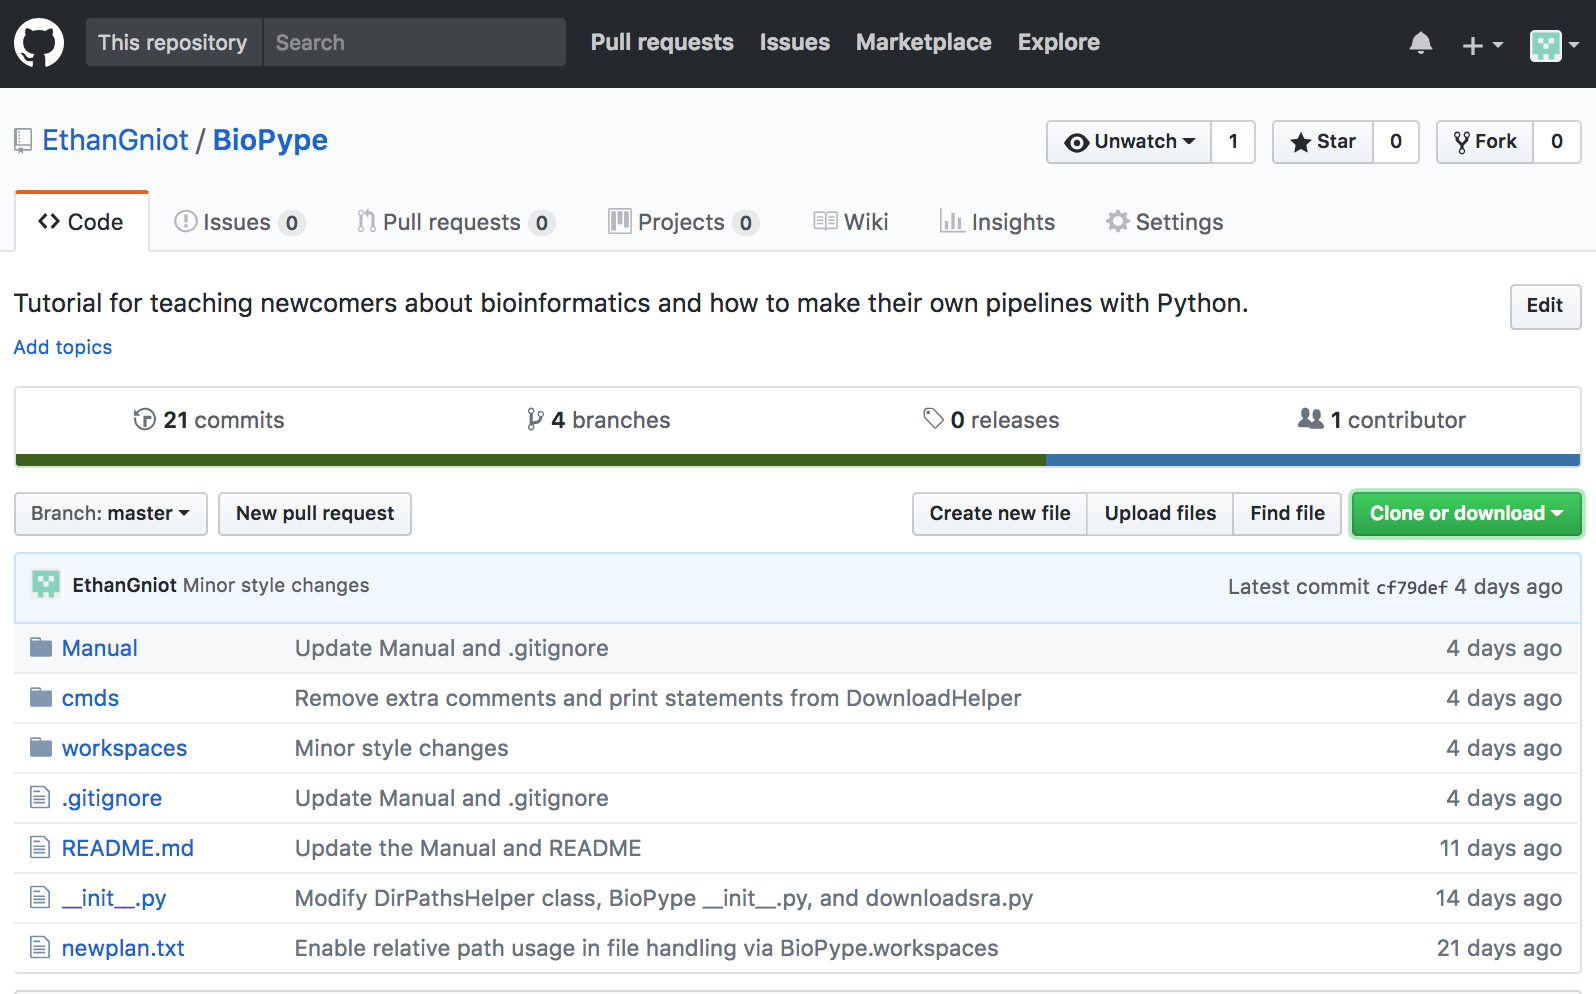
\includegraphics[height=8.5cm, width=13cm]{biopype-github}
    \caption{The BioPype Github webpage.}
    \label{fig:biopype-github}
    \hrule
    \end{maxipage}
\end{figure}


\item Click on the "biopype-dependencies.txt" file to view its contents. Next, right-click on the "Raw" button situated to the top-right of the text field and select "Save Link As...". Save the file to your Home folder (for most users, this should be the folder that shares your username). 


\item Open your computer's command-line application (on a Mac, this is the Terminal application). In the Terminal prompt, type the following and then press "Enter" (Note: the "\$" symbol represents the terminal prompt where you type. Do not actually type the \$):
    \begin{lstlisting} [basicstyle=\small, language=Python]
$ pwd
    \end{lstlisting}

The next line in the Terminal should then display a file path that represents your "current working directory". The current working directory is essentially the "folder" that your Terminal is currently looking at. It can see all the files and folders in that directory and access them by name if you ask it to. \seealso{For more information on navigating your files via the command-line, see Appendix \ref{appendix:command-line-navigate}. } For most users, this file path should lead to your home directory (e.g., /Users/your-username ). If the file path does not lead to your home directory, please read Appendix \ref{appendix:command-line-navigate} to learn how to change your current working directory to your home directory. 

\item Enter the following command in the Terminal prompt and then press "Enter":
    \begin{lstlisting} [basicstyle=\small, language=Python]
$ ls
    \end{lstlisting}

The Terminal should now display a list of all the files and folders in your current working directory. If you can't see the "biopype-dependencies.txt" file in the list, double-check that you downloaded it to your home directory. If you can see the file in the list, proceed to the next step.


\item To install all of the dependencies needed to run BioPype, enter the following into the command prompt:
    \begin{lstlisting} [basicstyle=\footnotesize, language=awk]
$ conda create --name biopype --file biopype-dependencies.txt
    \end{lstlisting}
The Terminal will take a while to think after you press "Enter" as it prepares to download all of the necessary packages. The different parts of this command accomplished several things:
    \begin{enumerate}
        \item \verb|conda|: this tells the Terminal that we want to execute one of conda's functions.
        \item \verb|create|: the conda function we want to use is the "create" function, which creates a new conda \textbf{virtual environment}. \seealso{For information on \textbf{virtual environments}, what they are, and why they're useful, see Appendix \ref{appendix:virtual-environments}.}
        \item \verb|--name|: this tells the Terminal that we are about to tell it what to name the new virtual environment.
        \item \verb|biopype|: this is the name of the new virtual environment.
        \item \verb|--file|: this tells the Terminal that we are about to tell it the name of a file containing dependencies that we want it to use when creating the new environment.
        \item \verb|biopype-dependencies.txt|: this is the name of the file containing the dependencies.
    \end{enumerate}
    After the terminal finishes thinking you will see the normal empty command prompt again. You should now have all of BioPype's dependencies installed in the "biopype" virtual environment. 


\end{enumerate}


\subsection{Installing dependencies with Anaconda}
This method is longer than the Miniconda method, so it will be broken up into three sections: 1) Installing and opening Anaconda, 2) creating a new virtual environment, and 3) installing dependencies.

\subsection*{Installing and Opening Anaconda}

\begin{enumerate}
    \item Go to the download page for the Anaconda distribution at \\ \url{https://www.anaconda.com/download}. 
    \item Select your preferred operating system from the Windows, macOS, or Linux tabs, then select the Download option for the \textbf{Python 3.6 version} (Figure \ref{anaconda_download}) and follow the installation instructions.

\begin{figure}[hbtp]
    \begin{maxipage}
    \hrule
    \centering
    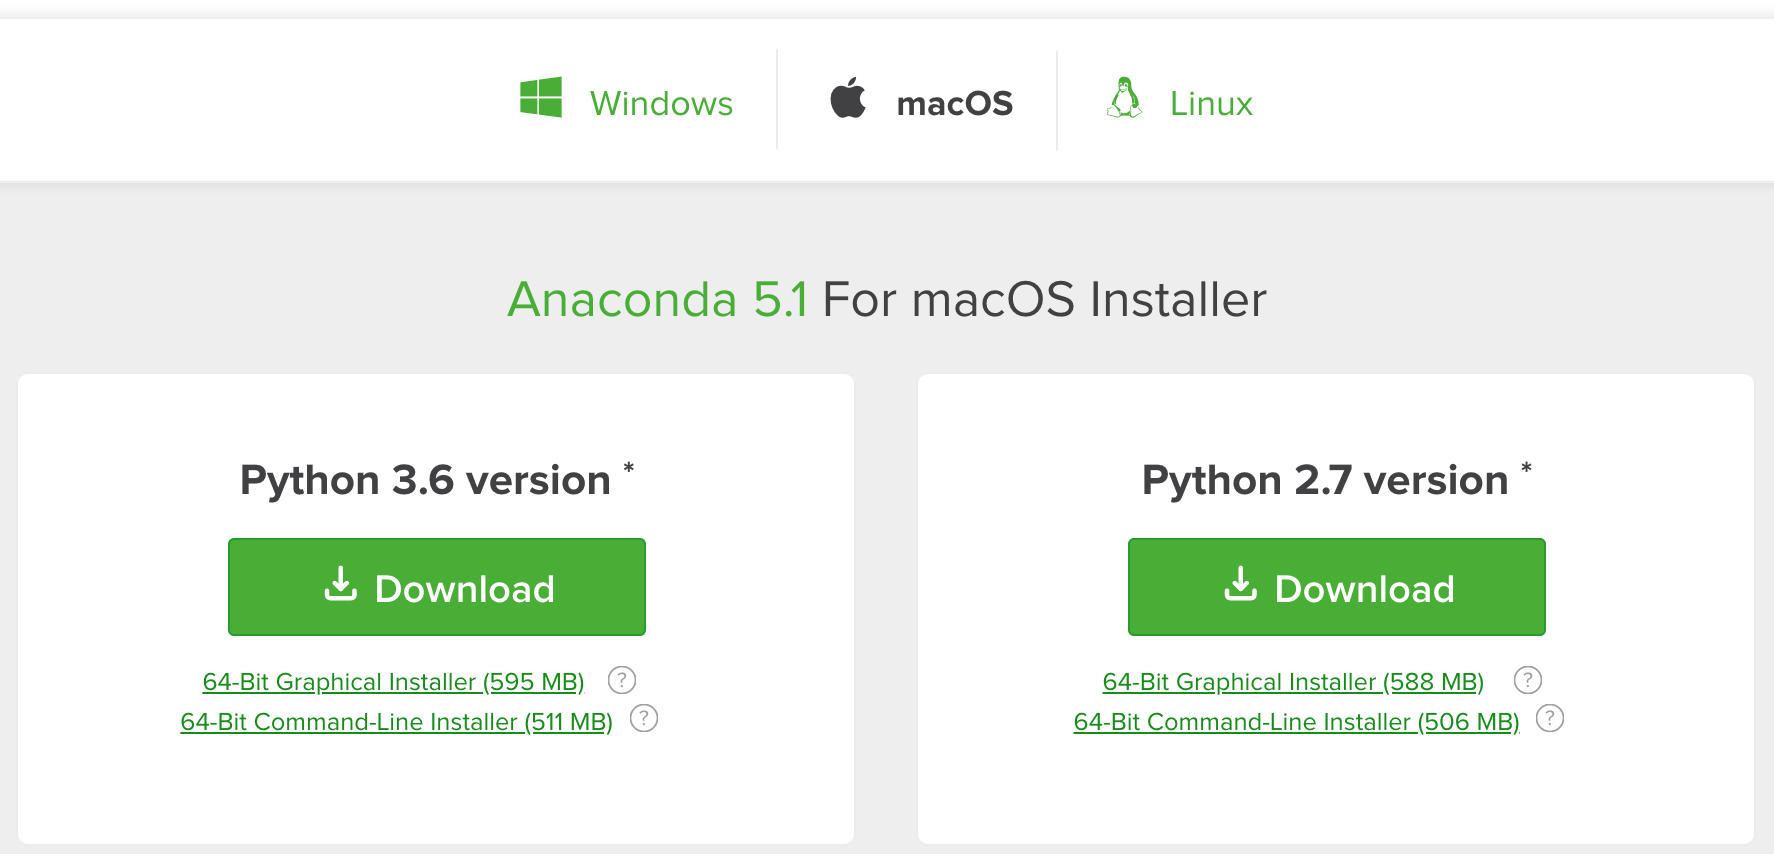
\includegraphics[height=5cm, width=9.5cm]{anaconda_download}
    \caption{The Anaconda download options provided on the Anaconda distribution website at \protect \url{https://www.anaconda.com/download}.}
    \label{anaconda_download}
    \hrule
    \end{maxipage}
\end{figure}


    \item After installation is complete, open the application named "Anaconda-Navigator" (the icon looks like 
\includegraphics[width=0.5cm]{anaconda-navigator-thumbnail}). After a brief start-up period, you should see the following window (Figure \ref{anaconda-nav-win}):
    
\begin{figure}[hbtp]
    \begin{maxipage}
    \hrule
    \centering
    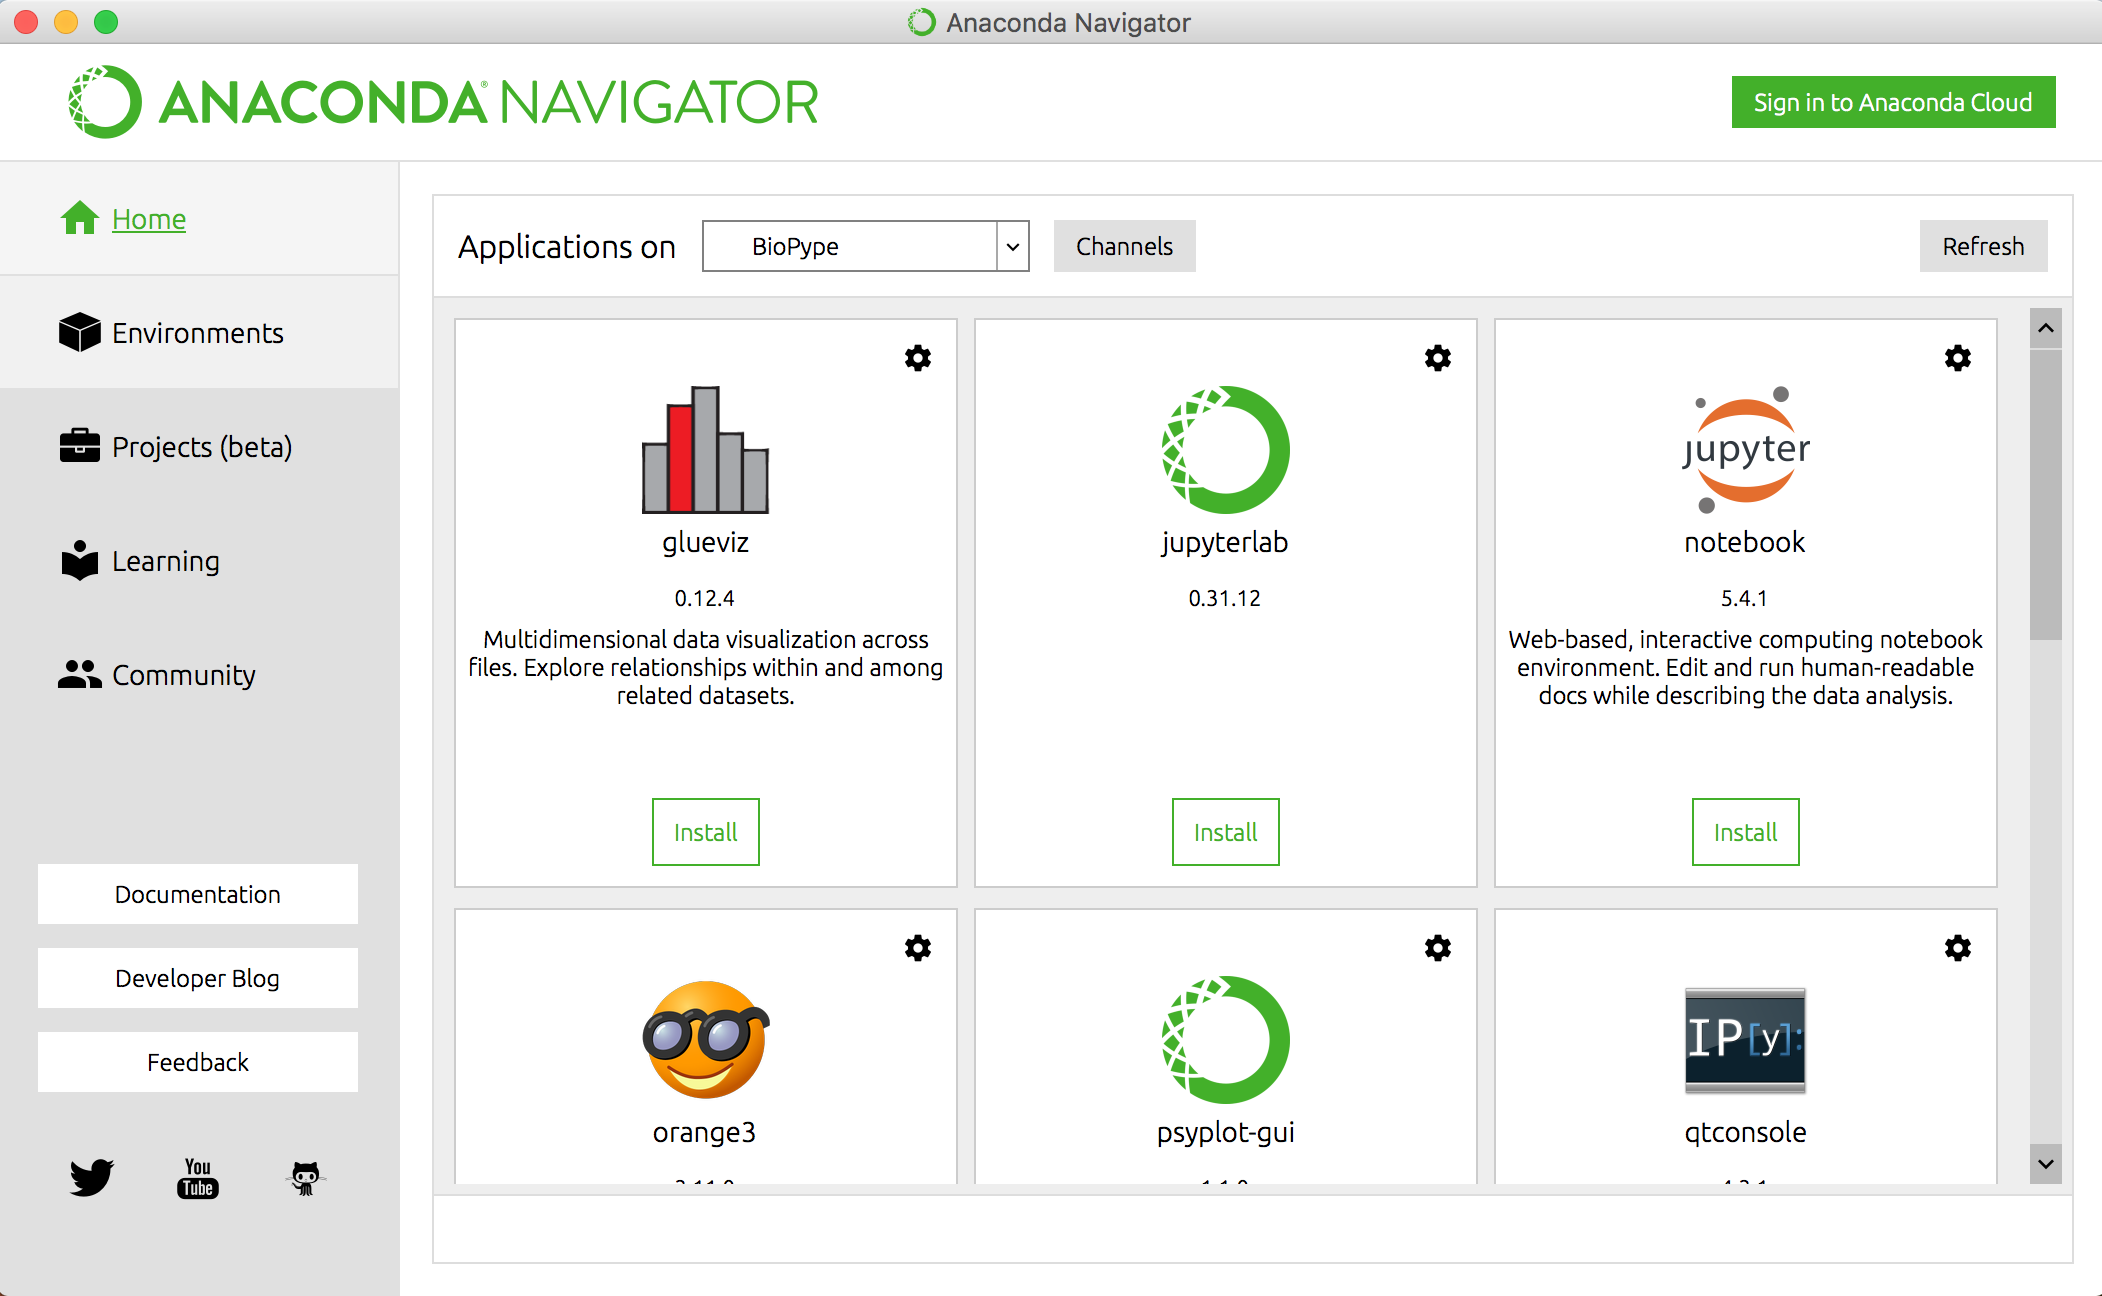
\includegraphics[height=7cm, width=11cm]{anaconda-nav-win}
    \caption{The window displayed to the user upon opening Anaconda-Navigator.}
    \label{anaconda-nav-win}
    \hrule
    \end{maxipage}
\end{figure}
    
    
\end{enumerate}

\subsection*{Create a New Virtual Environment}
    \todo[inline]{Link to resource for further reading on virtual environments}
    
    \begin{enumerate}
        \item \marginlabel{Make sure the computer has an internet connection while completing this section, otherwise Anaconda will not let you create a virtual environment.} On the left side of the Anaconda-Navigator window, click on the tab labeled \textbf{Environments}. (Figure \ref{anaconda-env-win}) 
        
\begin{figure}[hbtp]
    \begin{maxipage}
    \hrule
    \centering
    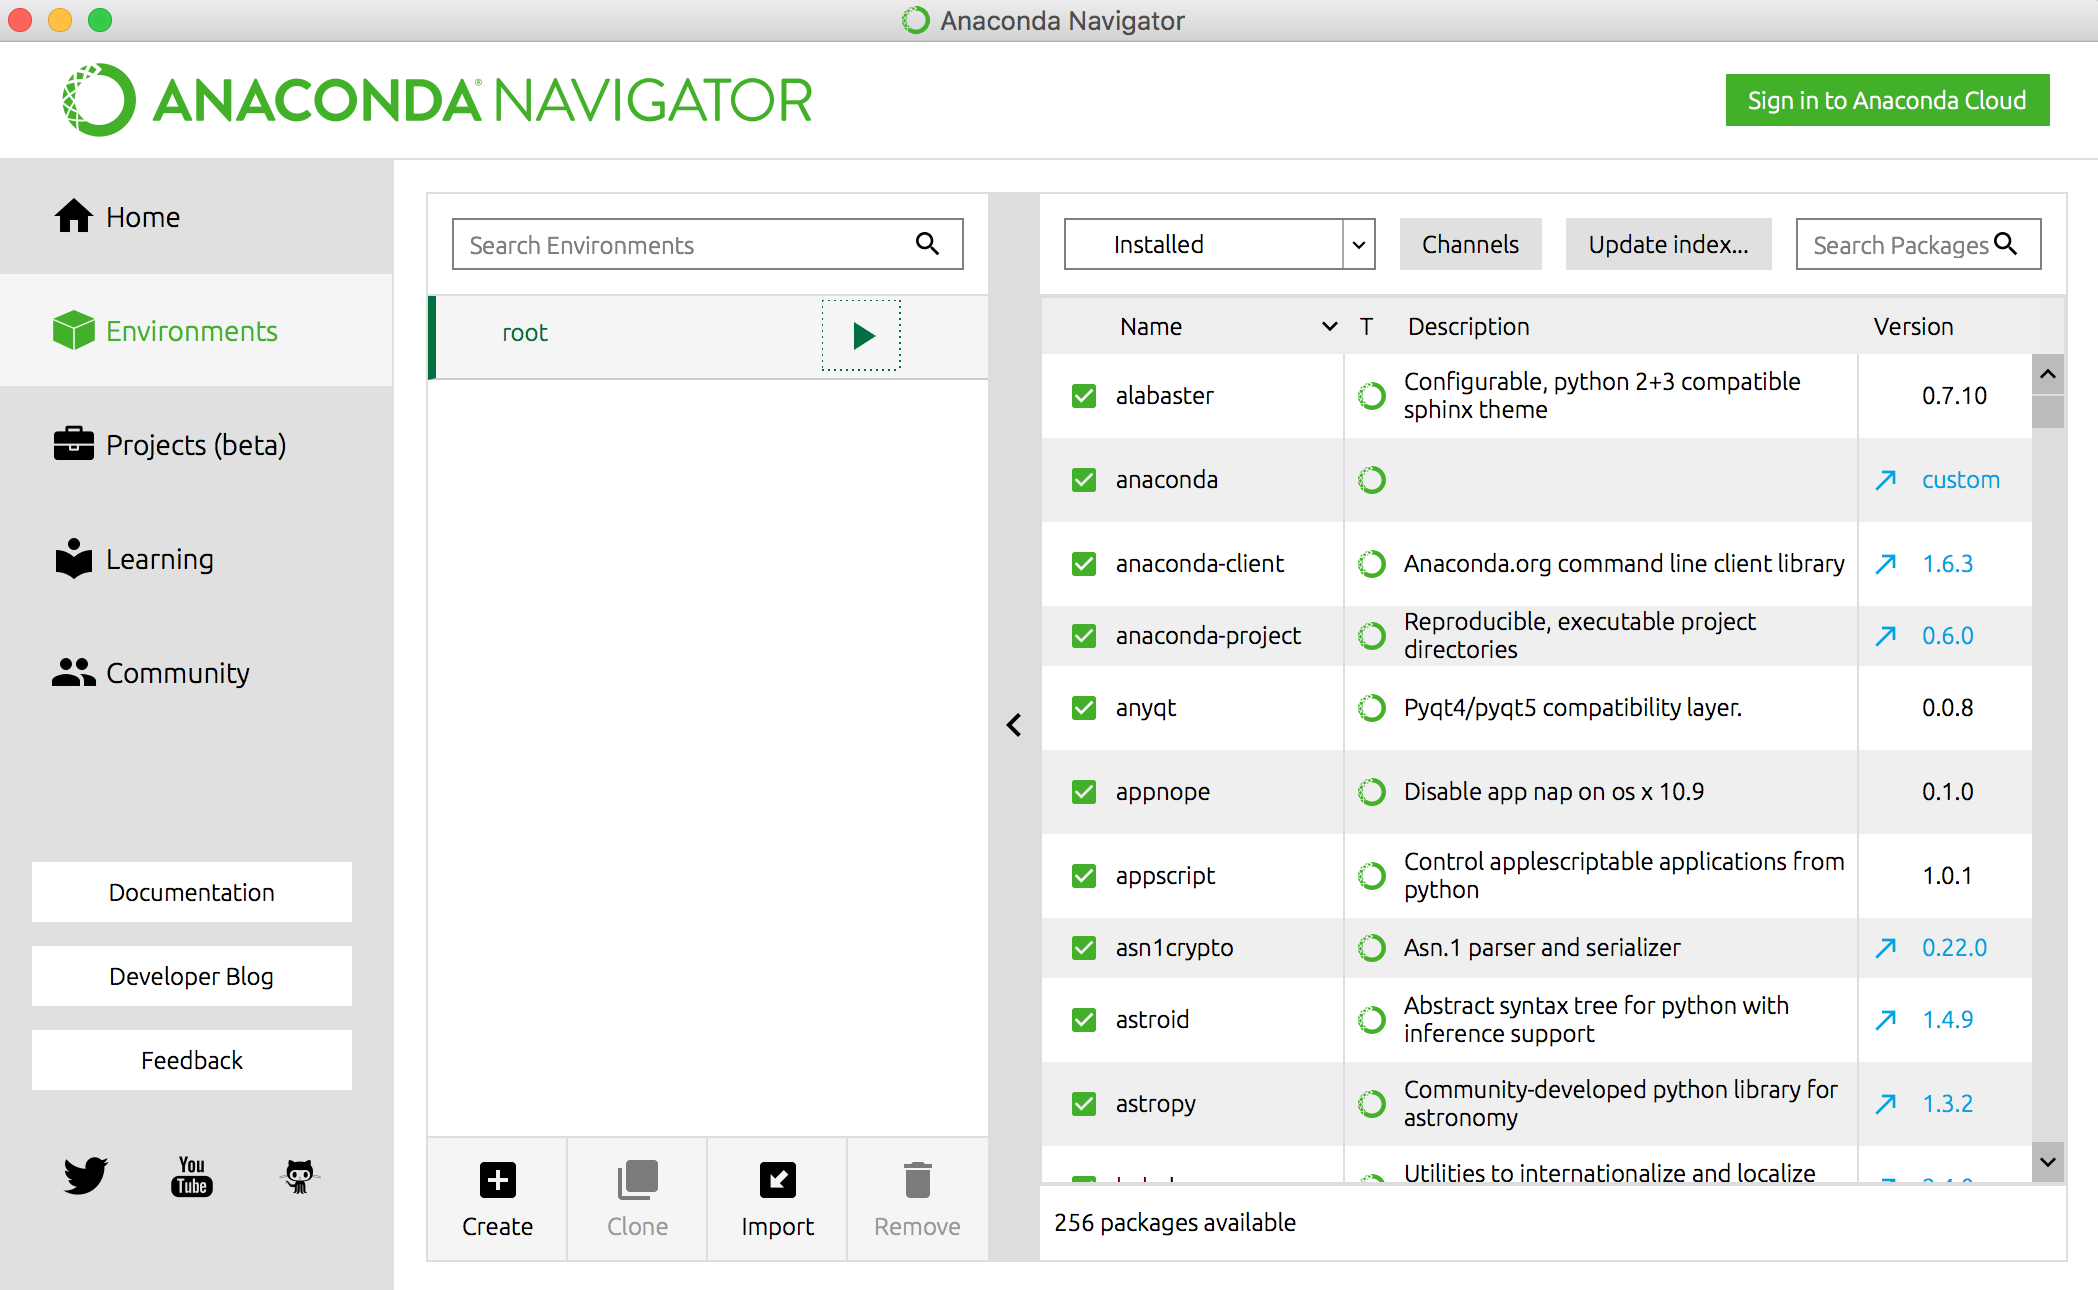
\includegraphics[width=12cm]{anaconda-env-win}
    \caption{The Environments window of the Anaconda-Navigator.}
    \label{anaconda-env-win}
    \hrule
    \end{maxipage}
\end{figure}
        \item Click the \textbf{Create} button on the bottom of the center panel. A new window titled "Create new environment" will appear. (Figure \ref{anaconda-create-new-env-win})

\begin{figure}[hbtp]
    \begin{maxipage}
    \hrule
    \centering
    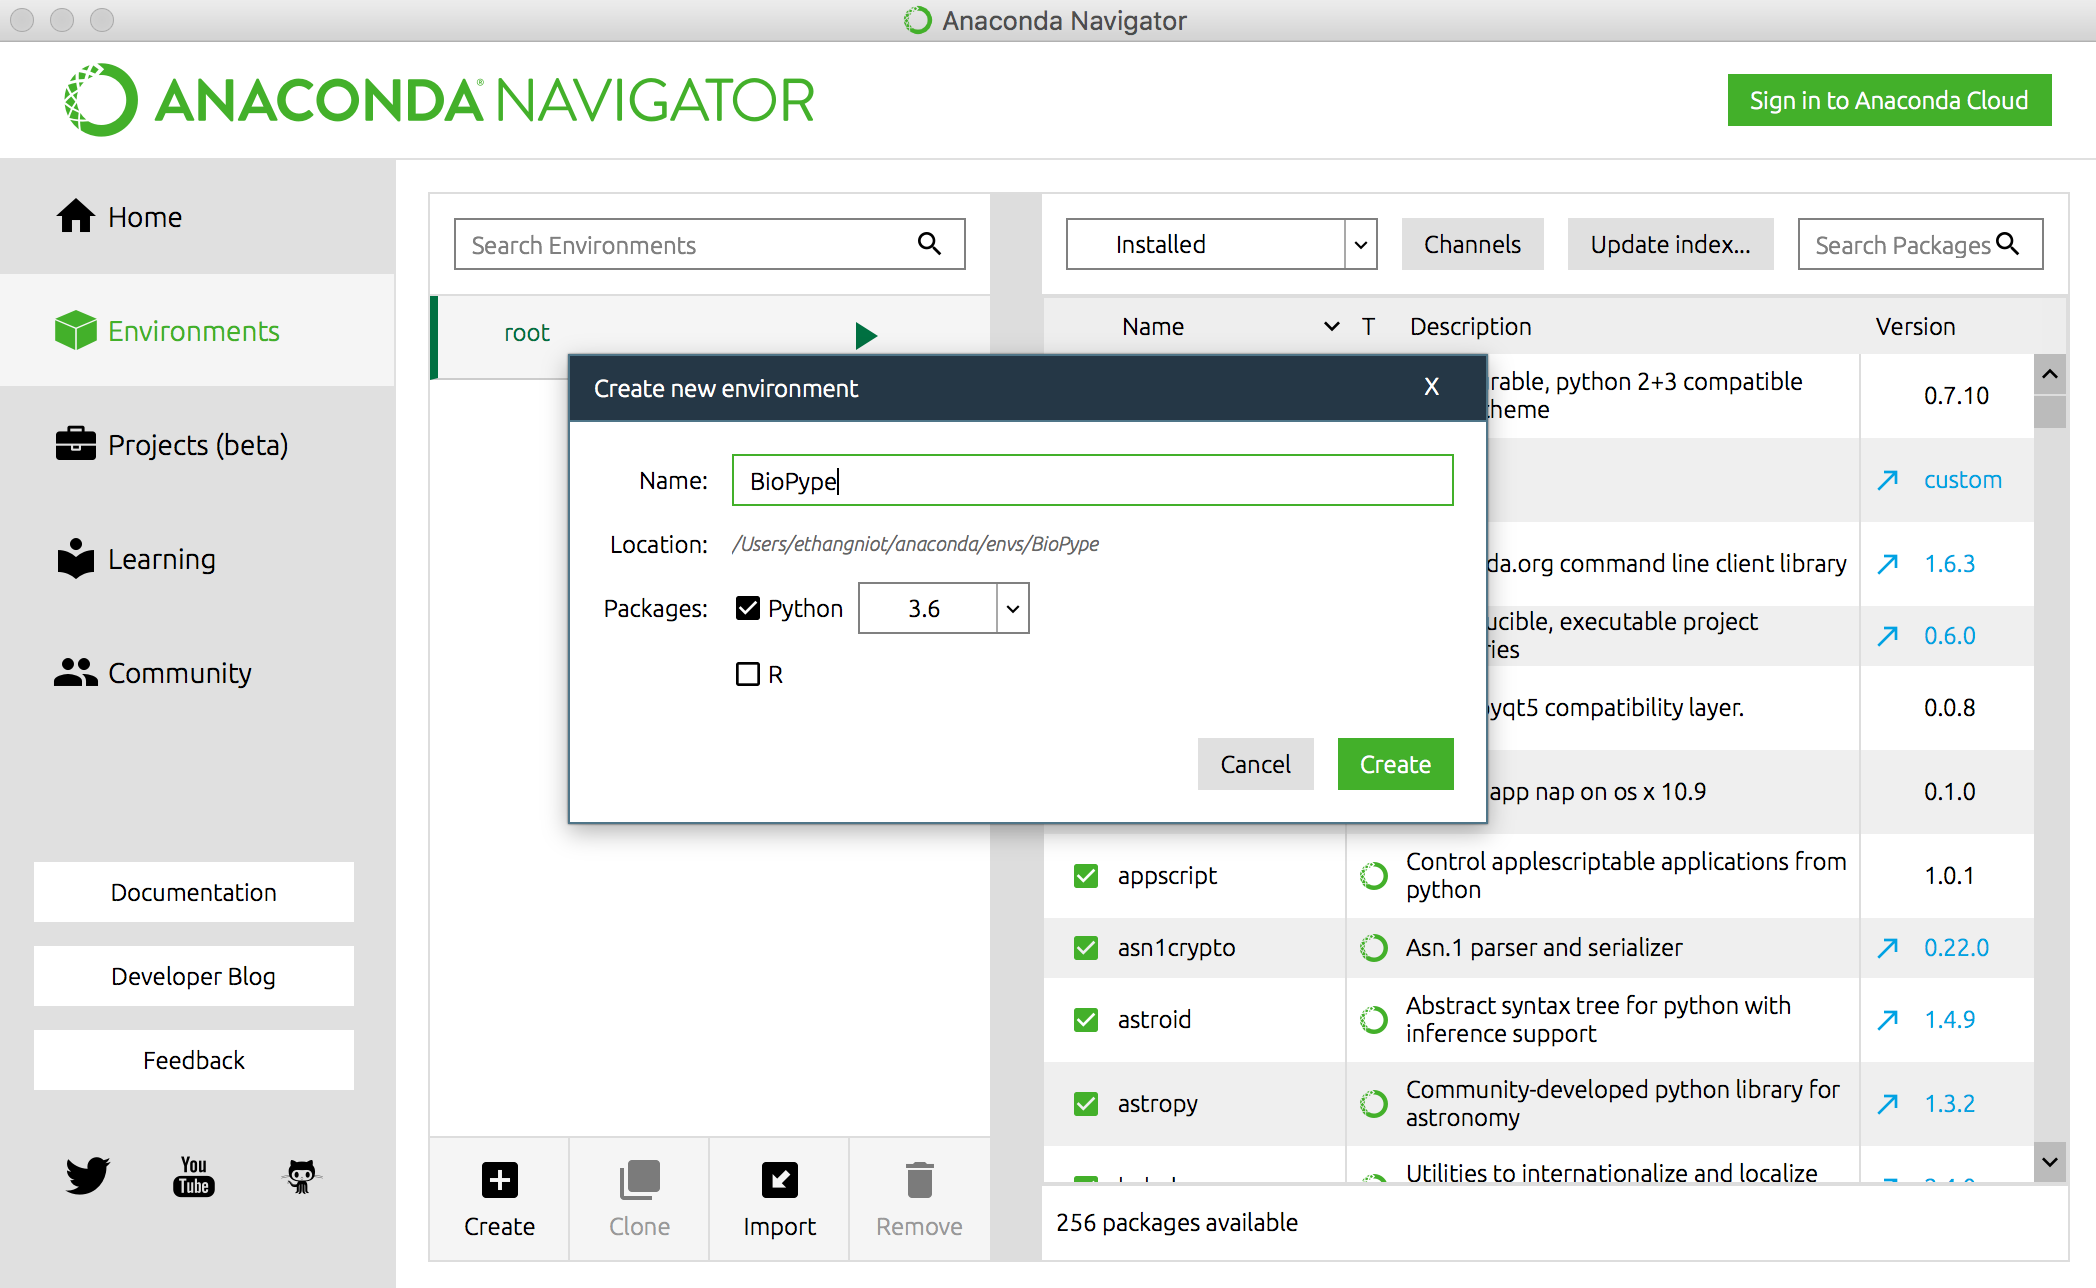
\includegraphics[width=12cm]{anaconda-create_new_env_win}
    \caption{The "Create new environment" window.}
    \label{anaconda-create-new-env-win}
    \hrule
    \end{maxipage}
\end{figure}
        
        \item Enter a \textbf{Name} for the environment. You may choose any name you want, but for the sake of this tutorial we will name the new environment "biopype".
        \item Select the box labeled \textbf{Python} next to the \textbf{Packages} heading.
        \item Choose a version of Python from the adjacent drop-down menu (Python 3.6 is the most current version at the time of this writing, but the packages we use require Python 3.5 so we chose \textbf{3.5}. If you are following the tutorial analysis in this manual, choose version 3.5).
        \item Click the \textbf{Create} button within the "Create new environment window".
    \end{enumerate}

\subsection*{Install packages}
    \begin{enumerate}
        \item Change Anaconda's current environment from the \textbf{root} environment by selecting the \textbf{biopype} tab in the middle panel of the Environments window.
        \item Click on the drop-down menu in the right-hand panel that says "Installed" and change it to "All".
        \item In the "Search Packages" box we can search for the packages that BioPype needs in order to function. For instance, if BioPype depended on the "biopython" package, we could enter "biopython" into the box. The search should then return a package named "biopython". We would then select the checkbox to the left of the name. (Figure \ref{anaconda-search-pack})
        \begin{itemize}
            \item A pair of green and red boxes (reading "Apply" and "Clear", respectively) will appear in the bottom-right of the window once a package is selected. Do not click these just yet. 
    %

\begin{figure}[hbtp]
    \begin{maxipage}
    \hrule
    \centering
    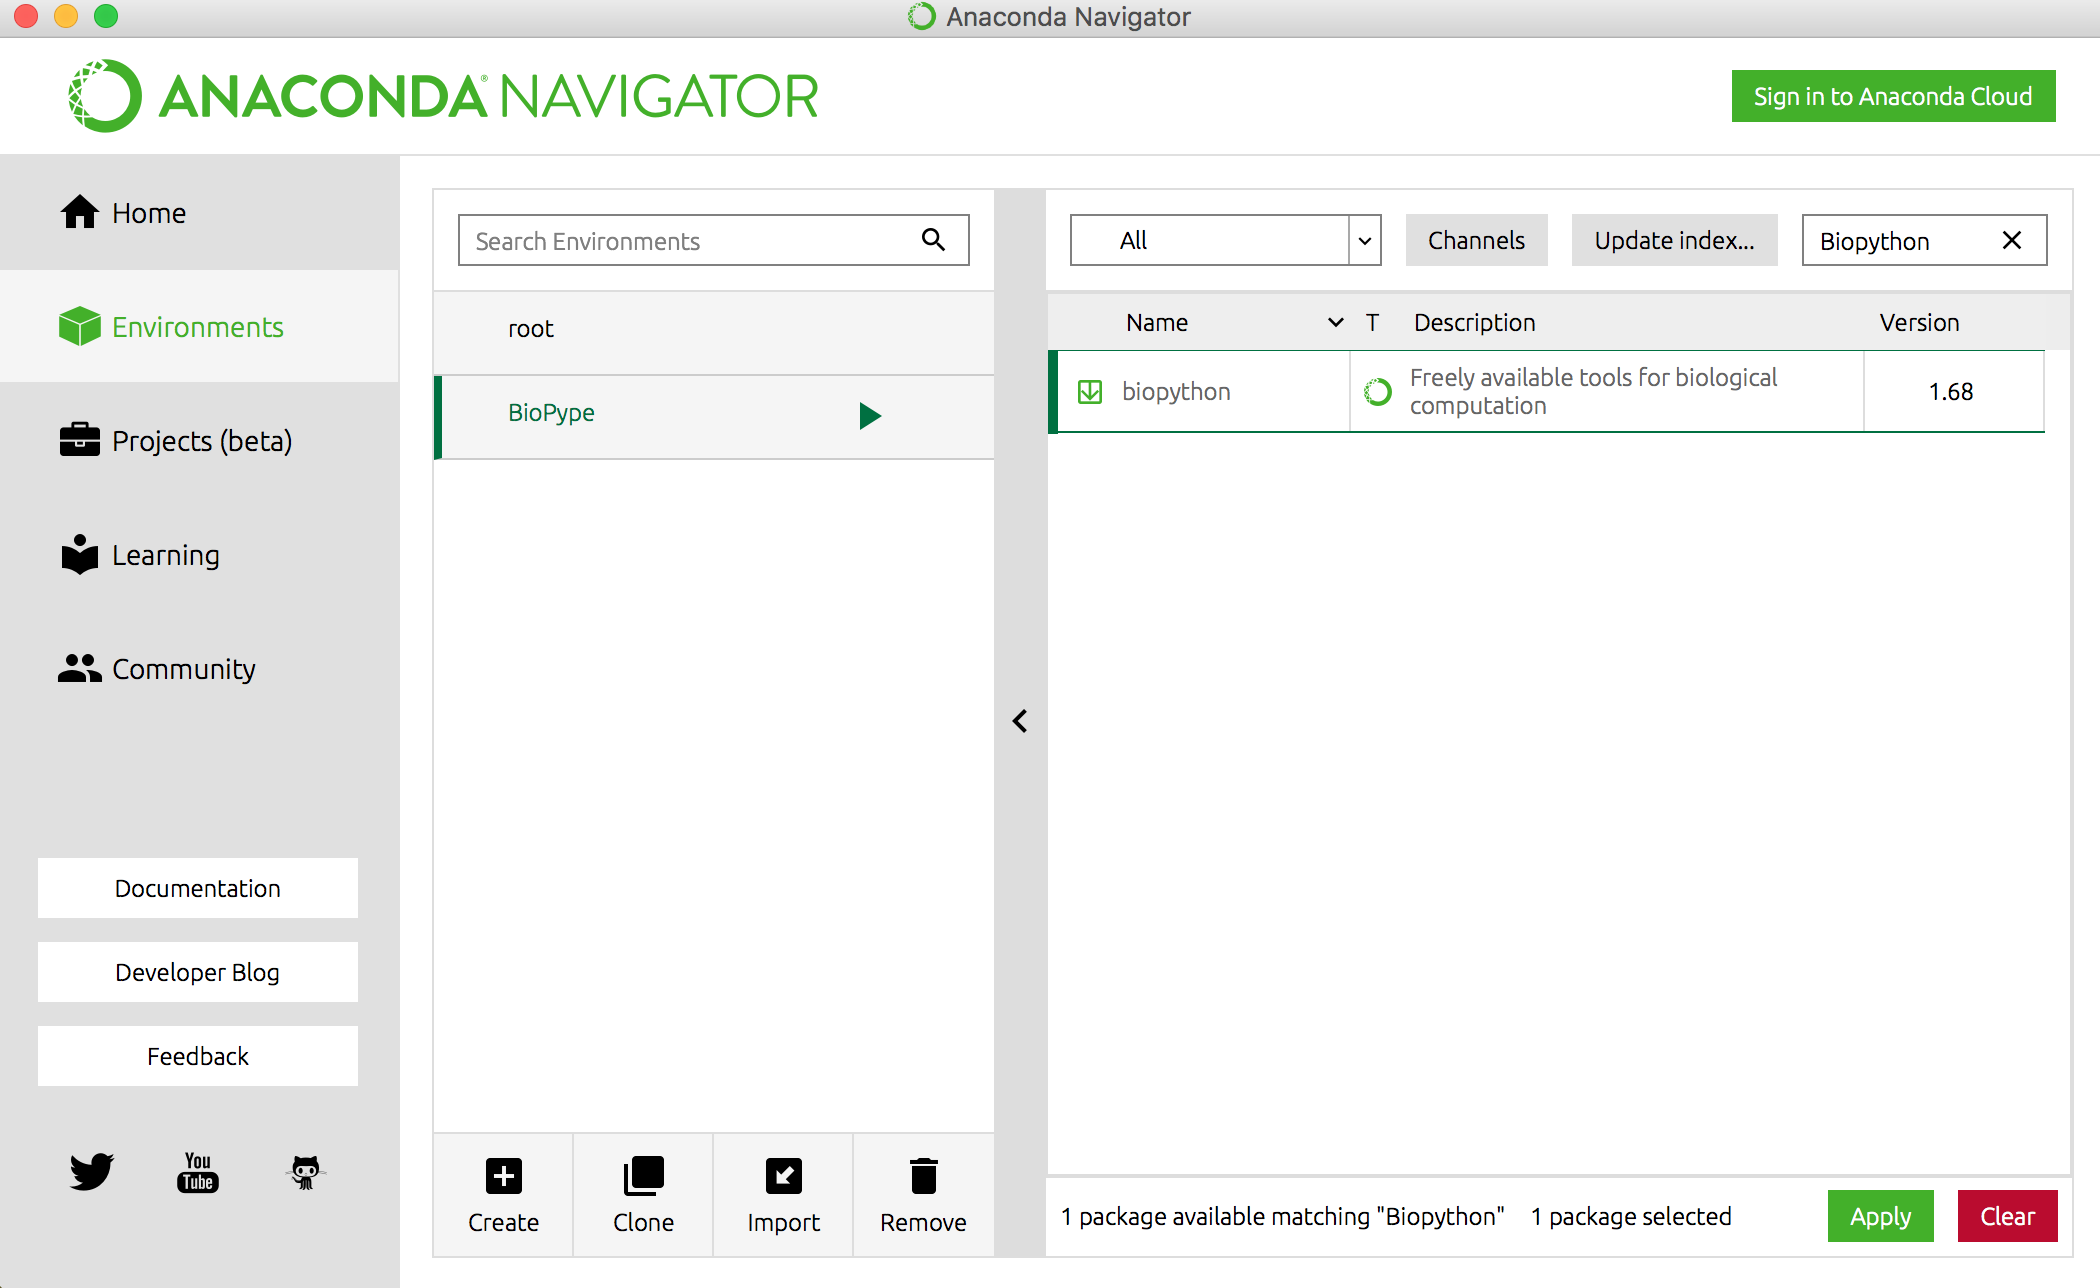
\includegraphics[width=12cm]{anaconda-search-pack}
    \caption{Searching for a package. When a package is selected, the checkbox next to the package's name will be green.}
    \label{anaconda-search-pack}
    \hrule
    \end{maxipage}
\end{figure}
    %
        \end{itemize}
        \item Use the search bar to find and select the packages listed in \autoref{tab:software} (except qiime2. That will need to be added to the environment by obtaining the .yml file from the qiime2 installation link and using the \verb|conda env install --name <env-name> --file qiime2-2018.4-py35-osx-conda.yml| command). Once all packages have been selected, click the green "Apply" button in the bottom right corner of the window, then select "Apply" again within the "Install Packages" window that appears. (Figure \ref{anaconda-install-pack}) Anaconda will now install the selected packages.
        \begin{itemize}
        \item Note: it may take a while for the windows to fully load when selecting "Apply" and "Install Packages", due to so many being selected at a time. 
        \end{itemize}
    %

\begin{figure}[hbtp]
    \begin{maxipage}
    \hrule
    \centering
    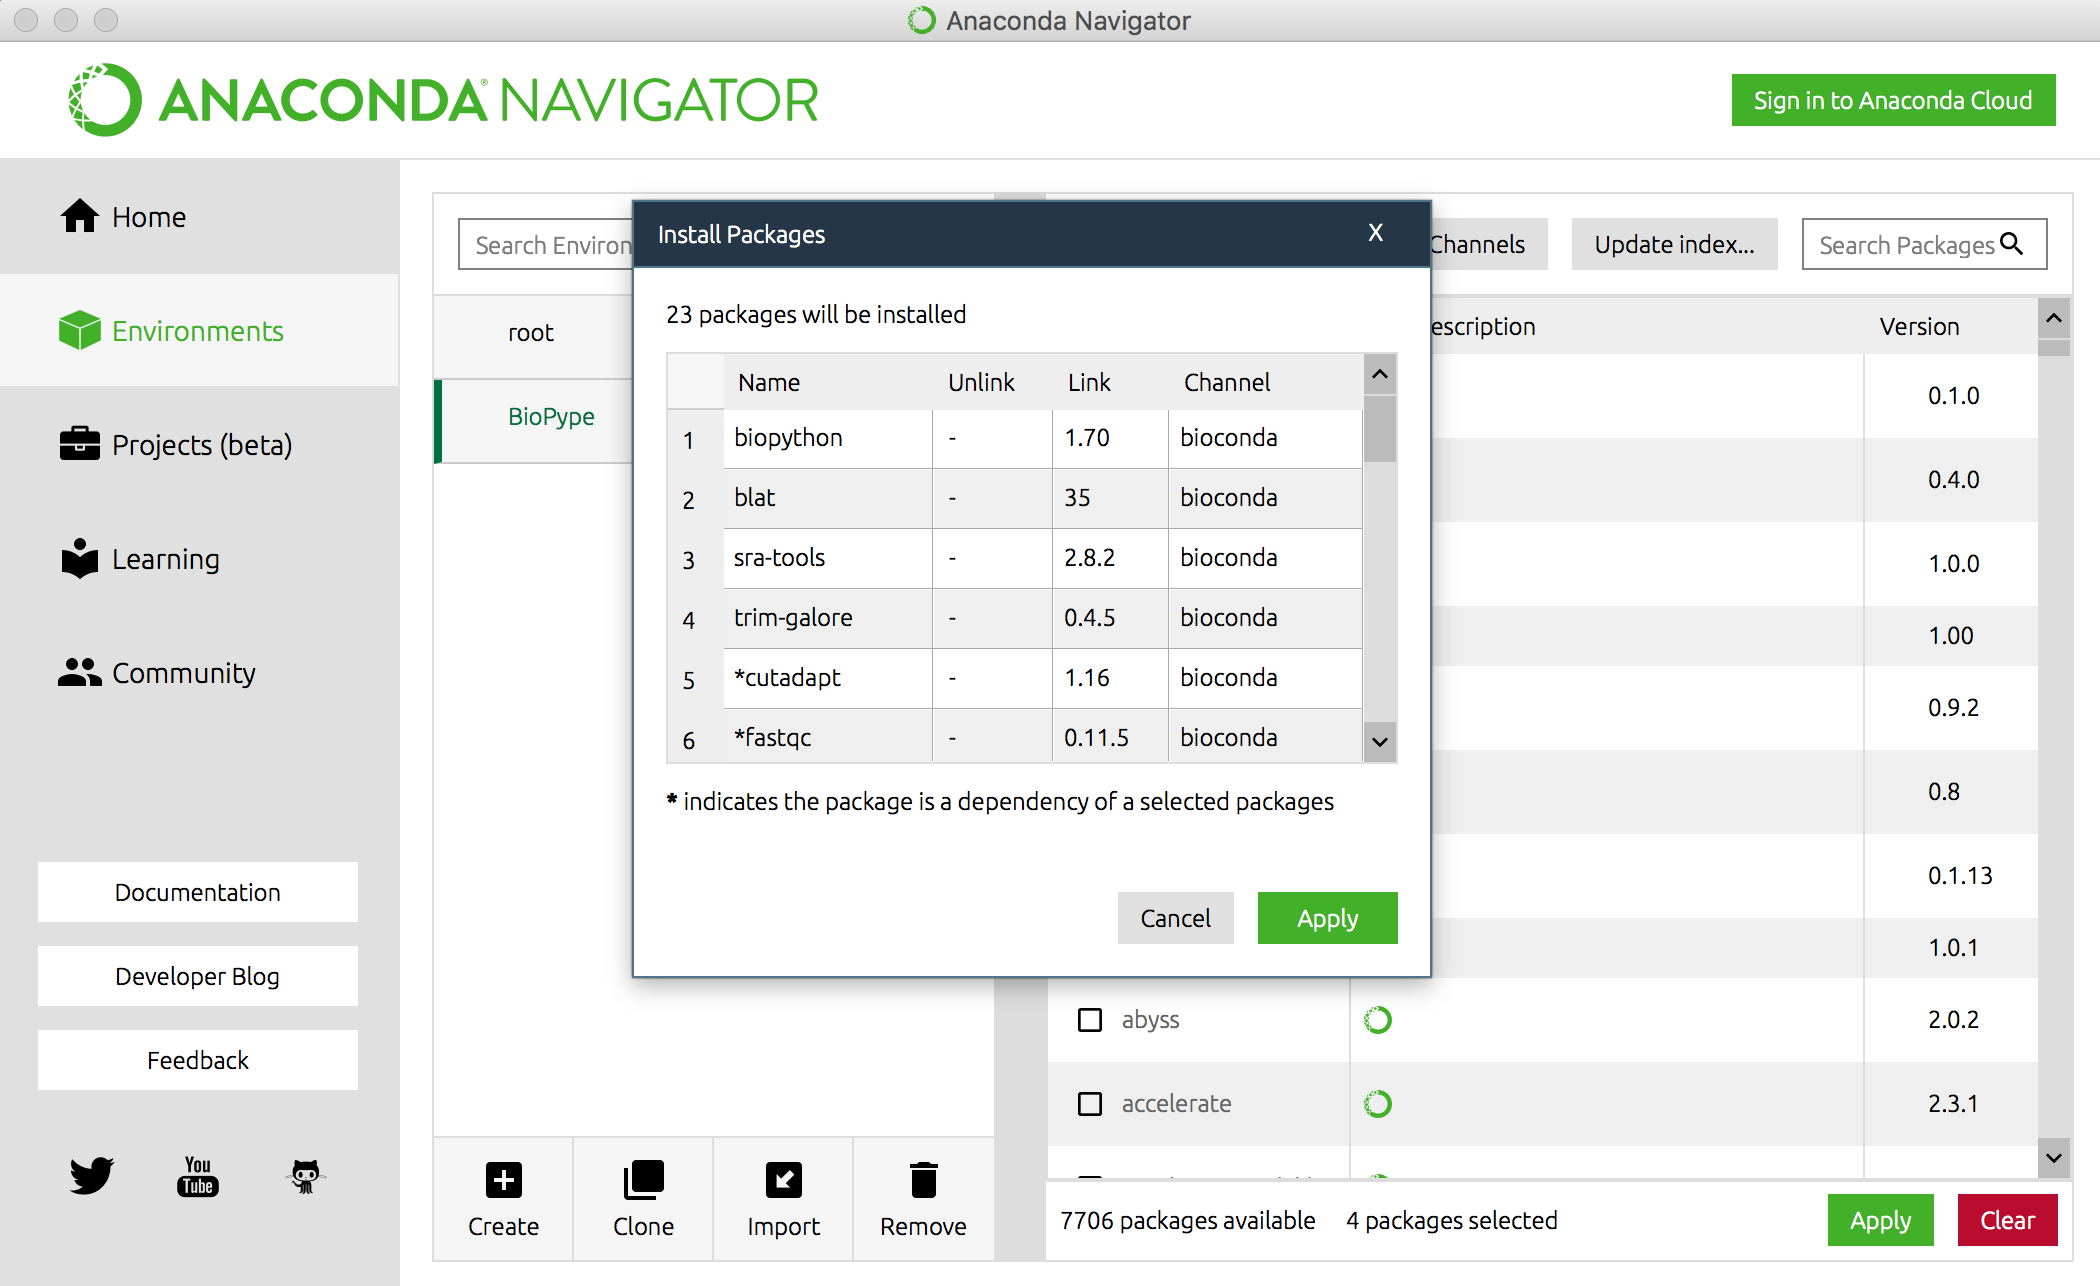
\includegraphics[width=12cm]{anaconda-install-pack}
    \caption{The window displaying the packages and dependencies that will be installed.}
    \label{anaconda-install-pack}
    \hrule
    \end{maxipage}
\end{figure}
    
    \end{enumerate}


\subsection{Downloading BioPype}

With the dependencies installed, we now need to download BioPype. 

\begin{enumerate}
\item Go back to the BioPype Github repository at \url{https://github.com/EthanGniot/BioPype}. (See Figure \ref{fig:biopype-github}).

\item Click on the green "Clone or download" button (see Figure \ref{fig:biopype-github})
    \begin{itemize}
    \item \small Note: The Github page that the URL from step 1 brings you to contains the code for the most recent "master" update to the BioPype repository. The "master" updates are usually the most recent \textit{stable} versions of BioPype. However, there may also be other versions of BioPype that are newer, but may contain bugs due to being under active development. To access these versions, click on the "branches" link (in Figure \ref{fig:biopype-github}, it is the link that says "4 branches" next to a branching symbol). If there are any branches (i.e., "versions") of BioPype that are more-current than the "master" branch, you will be able to see them on this page. This page also has links to the branches, where you can download that version of the BioPype code.
    \end{itemize}
%
\item Click on the "Download ZIP" button (the blue button in Figure \ref{fig:biopype-download}).
    \begin{figure}[hbtp]
        \begin{maxipage}
        \hrule
        \centering
        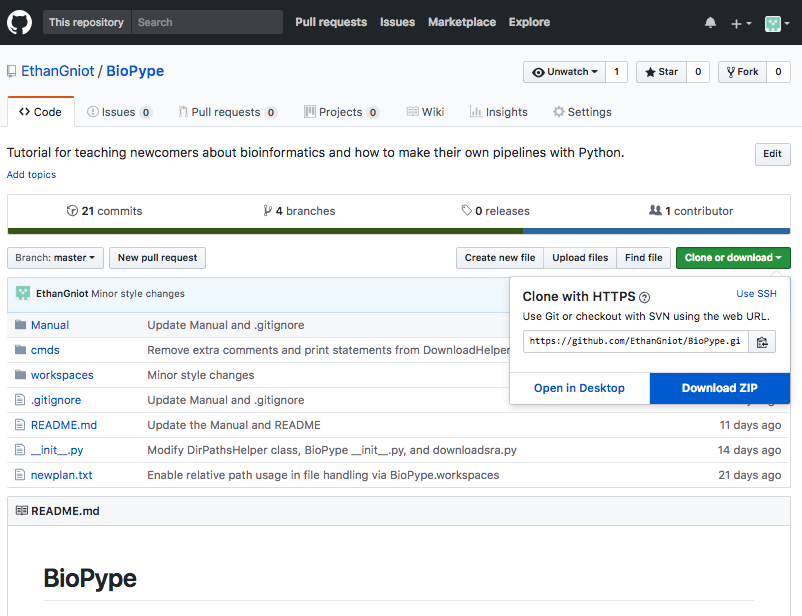
\includegraphics[height=8.5cm, width=13cm]{biopype-download}
        \caption{The button to download the BioPype code repository as a .zip file.}
        \label{fig:biopype-download}
        \hrule
        \end{maxipage}
    \end{figure}
    

\item Navigate to your Downloads folder and unzip the BioPype .zip file. 


\item Copy the BioPype folder, then navigate to the following file path and paste the folder into the "site-packages" folder (note: the parts of the file path that are in parentheses are not the literal names of directories. Substitute the appropriate directory into those spots based on the name of your home folder and whether you chose Anaconda or Miniconda):\newline
(home-folder)/(Anaconda-or-Miniconda)/envs/biopype/lib/python3.5/site-packages

\end{enumerate}


%
\subsection{The BioPype Project Directory and the SRA Toolkit Workspace Location}
To perform a microbiome analysis with BioPype, we will need a location where we can save our data and files. 
\begin{enumerate}

\item \marginlabel{\small The \textbf{SRA database} is a place where researchers can upload the sequencing data they use in their experiments for public access. Along with the raw sequence data, they also provide information about the experimental methods they used in the study that the sequencing data come from. } Create a directory somewhere in your file system and name it \newline "biopype\_project". (Remember that microbiome sequencing files are very large, so make sure to create the project folder somewhere with a lot of free storage space.) 

One of the packages BioPype uses is the SRA Toolkit (the package name in your file system will be "sra-tools"). This package lets us download .sra files from the NCBI \textbf{Sequence Read Archive (SRA) database}. In order to use the package, it requires that a directory called the "Workspace Location" be configured first. 

\item Create a folder inside the \verb|biopype_project| directory called "data".
\item In the Terminal, navigate to the "bin" subdirectory of the sra-tools package using the \verb|cd <path-to-subdir>| Terminal command.
\begin{itemize}
\item The bin subdirectory will be \textit{very} deep in your file system. The following file path is where the subdirectory is located on my machine:\newline /Users/ethangniot/miniconda3/envs/biopype\_project/share/ncbi\\/sra-tools/mac/clang/x86\_64/rel/bin
\end{itemize}

\item In your web browser, go to \url{https://trace.ncbi.nlm.nih.gov/Traces/sra/sra.cgi?view=toolkit_doc&f=std#s-4} and follow the configuration instructions to change the Workspace Location to the "data" folder you created in the \verb|biopype_project| folder.

\item In the Terminal, navigate back to the biopype\_project folder.


\item Activate the "biopype" virtual environment by typing the following into the command prompt:
\begin{lstlisting} [language=awk]
$ source activate biopype
\end{lstlisting}

\item Activate the Python interpreter by typing the following into the command prompt:
\begin{lstlisting} [language=awk]
$ python3
\end{lstlisting}

\item Import BioPype into the current Python environment:
\begin{lstlisting} [language=python]
>>> import BioPype
\end{lstlisting}


\item Upon importing BioPype, you should see a prompt appear in the Terminal window telling you what the current working directory for BioPype is, as well as the current Workspace Location for the SRA Toolkit. To change the location of where BioPype thinks these directories are, enter the following command:
\begin{lstlisting} [language=python]
>>>BioPype.path_helper.setup('biopype')
\end{lstlisting}

\item The Terminal will now ask you to "input a path to an existing folder to define BioPype's working directory". Input the file path to the "biopype\_project" folder. (e.g., /Users/username/biopype\_project)

\item Once the previous command is finished running, execute the following:
\begin{lstlisting} [language=python]
>>>BioPype.path_helper.setup('sra')
\end{lstlisting}
A prompt should appear that asks you to "input the path for the SRA Toolkit's configured Workspace Location." Input the path to the "biopype\_project/data" directory that you configured as the Workspace Location in step 4 of this section.


\end{enumerate}
%

The BioPype package should now be fully configured and ready to use for microbiome analyses!

%


